\subsubsection{CN3768}

Este módulo es el cargador de baterías, que utilizamos para cargar las tres. Se trata de un módulo con un controlador y un convertidor conmutado para generar la tensión de carga. 

El fabricante indica que acepta tensioens de entre $15 V$ y $24 V$, con una corriente de carga máxima de $4 A$, aunque la placa viene configurada para $200 mA$ con una resistencia, lo cual hemos respetado. Indica que la tensión de carga es de $14.8 V$ y que cuenta con una luz LED que debería indicar el estado de la carga. Sin embargo, hemos apreciado que el comportamiento de dicha luz es bastante poco constante, apagándose aleatoriamente durante el proceso de carga, aunque este siga en proceso. \cite{consonanceCN3768}

Un problema que no está indicado es la corriente en reversa. Este módulo cuenta con dos terminales de entrada y dos de salida. Cuando la tensión en los terminales de entrada es suficiente como para alimentar el módulo, se comporta adecuadamente y envía corriente a la batería para cargarla. Sin embargo, si la tensión en la entrada no es suficiente, el circuito permite corrientes en dirección contraria, descargando la batería. Esto lo hemos solucionado fácilmente con unos diodos \texttt{1N4007} en la entrada. Estos diodos cuentan con una corriente máxima de $1 A$ y una caída aproximada de $0.6 V$. Esta caída de tensión no nos afecta, ya que trabajamos bastante por encima de la tensión mínima de entrada del cargador.

\begin{figure}[h]
    \centering
    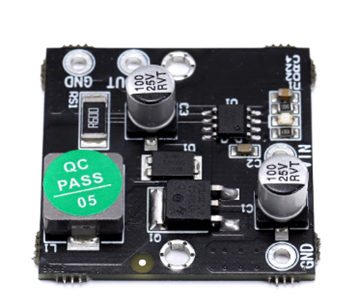
\includegraphics[width=0.5\textwidth]{images/2-hardware/componentes/CN3768.png}
    \caption{Módulo cargador \texttt{CN3768}}
    \label{fig:hardware/modulos/cn3768}
\end{figure}